\chapter{\LaTeX{} \index{\LaTeX} 的产生}{\LaTeX{} comes into being}
\TeX{} \index{\TeX} 还只是着重在于如何排版的层次上, 而不是从一位作者的立场出发. 对它深层功能的
进一步发掘, 需要相当丰富的编程技巧. 因此它的应用就局限于高级排版和程序设计人员.

虽然 \TeX{} \index{\TeX} 的功能很强大, 用它可以排版任何式样的文稿, 但普通用户要灵活掌握 \TeX{} \index{\TeX}
的 900 条初始命令还是有困难的. 因而, 在 \TeX{} \index{\TeX} 公开几年后, 利用 \TeX{} \index{\TeX} 的宏定义功能
开发的宏库 AMS\TeX{} 和 \LaTeX{} \index{\LaTeX} 就产生了.

AMS\TeX{} 是美国数学学会委托编写的, 主要用于美国数学学会及其分支机构出版的大量书籍、
期刊和评论. AMS\TeX{} 中含有一个宏包, 供作者用来方便地准备稿件. 用 AMS\TeX{} 可以
方便地排印出非常复杂的数学公式和 AMS 制定的全部数学符号.

\LaTeX{} \index{\LaTeX} 是由美国计算机学家 Leslie Lamport 于 1985 年开发成功的. 它是当今世界上最
流行和使用最为广泛, 以 \TeX{}\index{\TeX} 为引擎的高质量格式化排版系统. 它构筑在 \TeX{} 的基础
之上, 并且加进了很多新功能, 使得使用者可以更为方便的利用 \TeX{}\index{\TeX} 的强大功能. 使用
\LaTeX{}\index{\LaTeX} 基本上不需要使用者自己设计命令和宏等, 因为 \LaTeX{}\index{\LaTeX} 已经替你做好了. 因此,
即使使用者并不是很了解 \TeX\index{\TeX}, 也可以在很短的时间内制成高质量的文件. 对于排版复杂的
数学公式, \LaTeX{}\index{\LaTeX} 表现的更为出色.

\begin{figure}
  \centering
  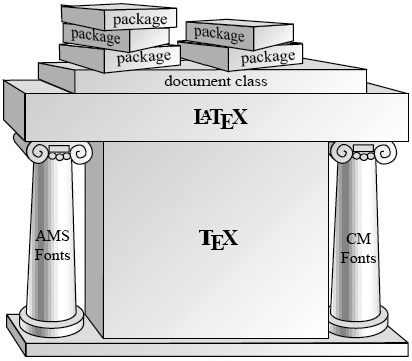
\includegraphics[width=8cm]{TexStone.png}\\
  \caption{\LaTeX{}\index{\LaTeX} 的结构示意图}{The structure of \LaTeX}
  \label{fig:TheStructureOfLaTeX}
\end{figure}


\TeX{}\index{\TeX} 是 \LaTeX{}\index{\LaTeX} 的基石, \LaTeX{}\index{\LaTeX} 建立在 \TeX{}\index{\TeX} 之上; 各种宏包和类型文件是 \LaTeX{}\index{\LaTeX}
大厦的装饰材料. \LaTeX{}\index{\LaTeX} 是特殊版本的 \TeX\index{\TeX}.

尽管在排版数学公式和数学符号方面, \LaTeX{}\index{\LaTeX} 不如 AMS\TeX, 但是 \LaTeX{}\index{\LaTeX} 提供了大量
易于学习和使用的命令, 例如非常有用的交叉引用命令等, 都是 AMS\TeX 所不具备的. 因而,
\LaTeX{}\index{\LaTeX} 的用途更为广泛, 特别是在排版信件、书刊、诗集等方面更优于 AMS\TeX.

自从 \LaTeX{}\index{\LaTeX} 问世以来, 流传最广的版本是 \LaTeX{}2.09\index{\LaTeX}. 由于 \LaTeX{}\index{\LaTeX} 的众多优点,
在计算机科学、数学及相关学科得到迅速广泛地应用, 吸引了许多专家、爱好者并为其编写和
添加了各式各样的宏包和宏库, 例如 PostScript 字体处理、排版复杂数学公式的 AMS\LaTeX{} 等,
这使得 \LaTeX{}\index{\LaTeX} 的功能不断地扩充, 应用领域不断地扩大. 但是, 由于没有统一的宏包编写
规划和编写格式, 造成某些宏包的功能彼此接近, 而命令相互冲突, 同一个源文件在某种格式
的 \LaTeX{}\index{\LaTeX} 中能够完美运行, 而在另一种格式中就可能编译出错或结果有所不同. 很多网站
和编辑部为了处理不同来源的 \LaTeX{}\index{\LaTeX} 文件, 不得不置备各种格式的 \LaTeX{}\index{\LaTeX} 系统; 有些
宏包很难分辨出是为那种格式编写的, 还得反复尝试.

有鉴于此, TUG 专门成立了 \LaTeX{}3\index{\LaTeX} 项目小组, 负责研发一个用途更加广泛, 功能更为完
善, 用户更易使用的崭新版本: \LaTeX{}3\index{\LaTeX}. 这是一个长期艰巨的科研计划, 为了尽快扭转当
时的混乱局面, \LaTeX{}3\index{\LaTeX} 项目小组先在 1994 年推出过渡版本 \LaTeX{}2$\varepsilon$\index{\LaTeX}.
新旧版本最明显的区别在于源文件的第一条命令, \LaTeX{}2.09 \index{\LaTeX} 为:
\begin{verbatim}
  \documentstyle[选项, 宏包名]{文件类型名}
\end{verbatim}
方括号里两种个不同类型的选择项并存, 容易产生混淆; \LaTeX{}2$\varepsilon$ \index{\LaTeX} 将其一分为二:
\begin{verbatim}
  \documentclass[选项]{文件类型名}
  \usepackage{宏包名}
\end{verbatim}
而且宏包也可以有自己的选项.

字体处理是新版最重要的改进, 它将 NFSS 作为标准的字体选择方法, 可处理任意编码的字体,
而旧版仅支持 OT1 编码. NFSS 是用属性的方式描述字体, 因此可分别独立地选择字体的某种
属性, 例如先选黑体, 再选斜体, 从而得到黑斜体, 这在旧版本是不可能的事儿.

新版本把 SLiTeX、AMSLaTeX 等宏库都归为附属的扩展宏包套件, 并将其中所有宏包的命令格
式统一, 可以用命令调用; 它还对浮动体定位、命令语句功能等方面进行了改进或扩充, 并对
旧版本中的错误和漏洞作了修补. 新版本还增添了许多新的功能、命令和错误提示信息以及处
理多种文字的 babel 宏包套件、图形制作的 graphics 宏包套件等.

新版本的另一个重要改进就是提供了更为高效便捷的宏包文件或类型文件编写命令.

新版本兼容旧版本, 也就是说用 \LaTeX{}2.09 \index{\LaTeX} 创建的源文件仍可在 \LaTeX{}2$\varepsilon$ \index{\LaTeX}
中运行, 只是速度要慢一半, 因为要在两种模式中切换; 如想要加快并享受新版的乐趣, 须将
源文件第一条命令改为新版形式.

\begin{figure}
  \centering
  
\includegraphics[width=8cm]{LaTeX2e.png}\\
\end{figure}

\LaTeX{} \index{\LaTeX}的读法应为``lay-teck", 念成``lay-tecks"也可以.

\LaTeX{}2$\varepsilon$ \index{\LaTeX}可读作``Lay-teck two e".

\LaTeX{} \index{\LaTeX}的标准写法比它的读法更别致, 应该是上图中的样子, 这在 \LaTeX{}\index{\LaTeX} 源文件中使用
专有命令就可轻易做到, 而在网页上很难实现, 为了简便起见, 都采用目前这种非常规大写形
式, \LaTeX{}2$\varepsilon$ \index{\LaTeX}也被简化成 \LaTeX{}2$\mathrm{e}$\index{\LaTeX}.

在 \LaTeX{}3 \index{\LaTeX}最终完成之前, \LaTeX{}2$\mathrm{e}$ \index{\LaTeX}仍将是标准的 \LaTeX{}\index{\LaTeX} 版本, 由
\LaTeX{}3 \index{\LaTeX}项目小组负责维护.

更多关于 \LaTeX{} \index{\LaTeX}的资料可以参考
\citet*{OetikerPartlHynaSchlegl2007,Leslie1994,MittelbachGoossensBraamsCarlisleRowley2004,ChenZhiJie2006,HuWei2011}.
